\chapter{系统概要设计}

\section{技术方案介绍}


该应用在服务器端采用Node.js编写, 其好处是Web开发生态环境好, 现成的服务和工具多, 在这里我使用npm提供的 private node modules和github提供的付费 organization 的服务, 将整个大程序设计为由分成多个Node.js的模块组成。



\section{数据库架构设计}


下面

根据我们之前给的需求图, 我们设计出了我们的 mongodb数据库 架构。 见下图:

\newpage
l \newline
\begin{figure}[H]
	\centering
        \hspace*{-7cm}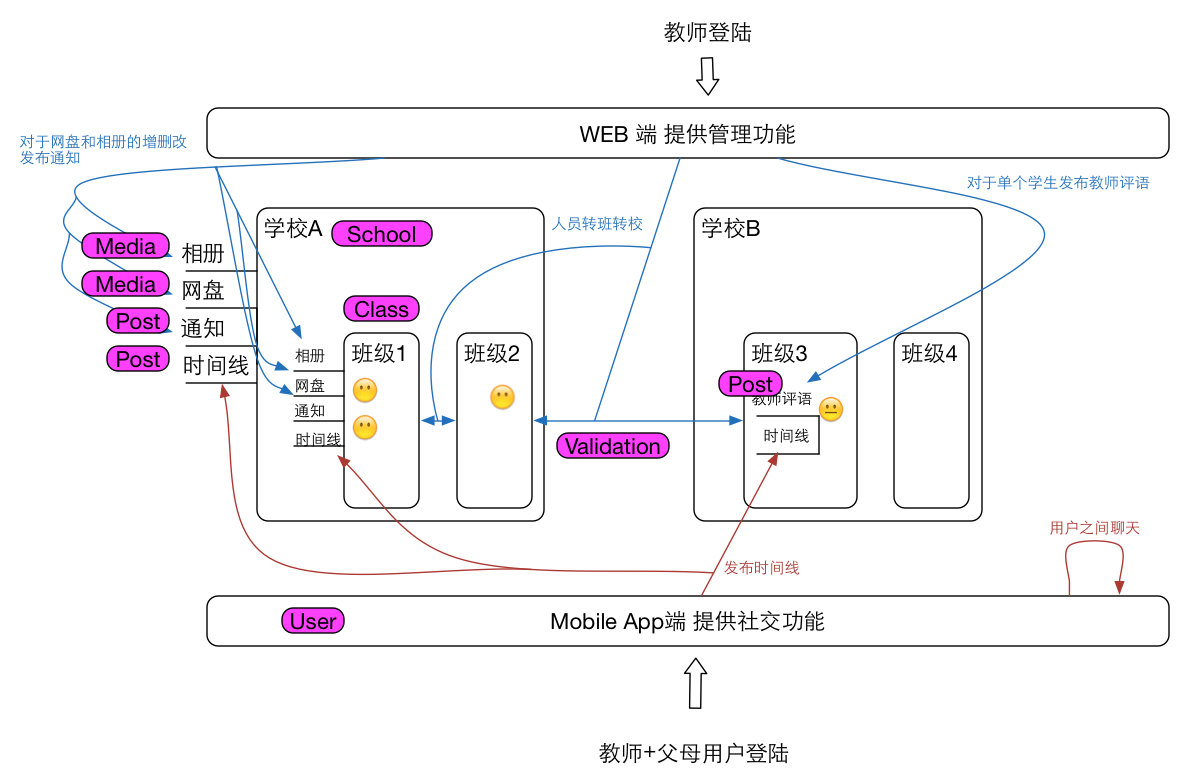
\includegraphics[width=\textwidth]{need-find-db.jpg}
	\figcaption{由业务流图而来的数据库设计}
	\label{fig:need-find-db}
\end{figure}

由上图可见, 其中紫色矩形部分为数据库中定义的model, 分别为:


\begin{description}
	\item[Post]  \hfill \\
	\thinspace 用户发布在时间线的状态
		\item[User]  \hfill \\
		\thinspace 用户模型
		\item[School]  \hfill \\
		\thinspace 学校模型
			\item[Class]  \hfill \\
			\thinspace 班级模型
			\item[Media]  \hfill \\
			\thinspace 文件模型, 用于网盘和相册
	\item[ValidationToken]  \hfill \\
	\thinspace 验证Token, 用于转班验证, 密码reset等

\end{description}


\section{系统后端功能架构设计}


\subsection{思路}

在系统后端, 我运行了两个服务器, 一个是普通的http服务器, 另一个是websocket服务器。 Http 服务器来处理普通的http请求, 并提供一些restful的接口。 websocket服务器和WEB端的管理用户建立socket连接, 实现双向的通信, 以达到

\begin{itemize}
	\item 更加安全
	\item 比ajax http请求更加快捷,高效
\end{itemize}





而这两个服务器提供的功能由一些node modules组成。 首先先要设计程序由哪些部分组成, 之后将这些部分设计为node modules。

\subsection{系统模块架构}

这里先给出 node modules的树形关系图, modules之间关系的设计借鉴了 java 中package命名空间的规范。 在给出关系图后, 会讲解每个module的功能, 和应当暴露出来的接口。node modules 树形关系图类似java程序的类图。

\newpage
\begin{figure}[H]
	\centering
	\vspace*{7cm}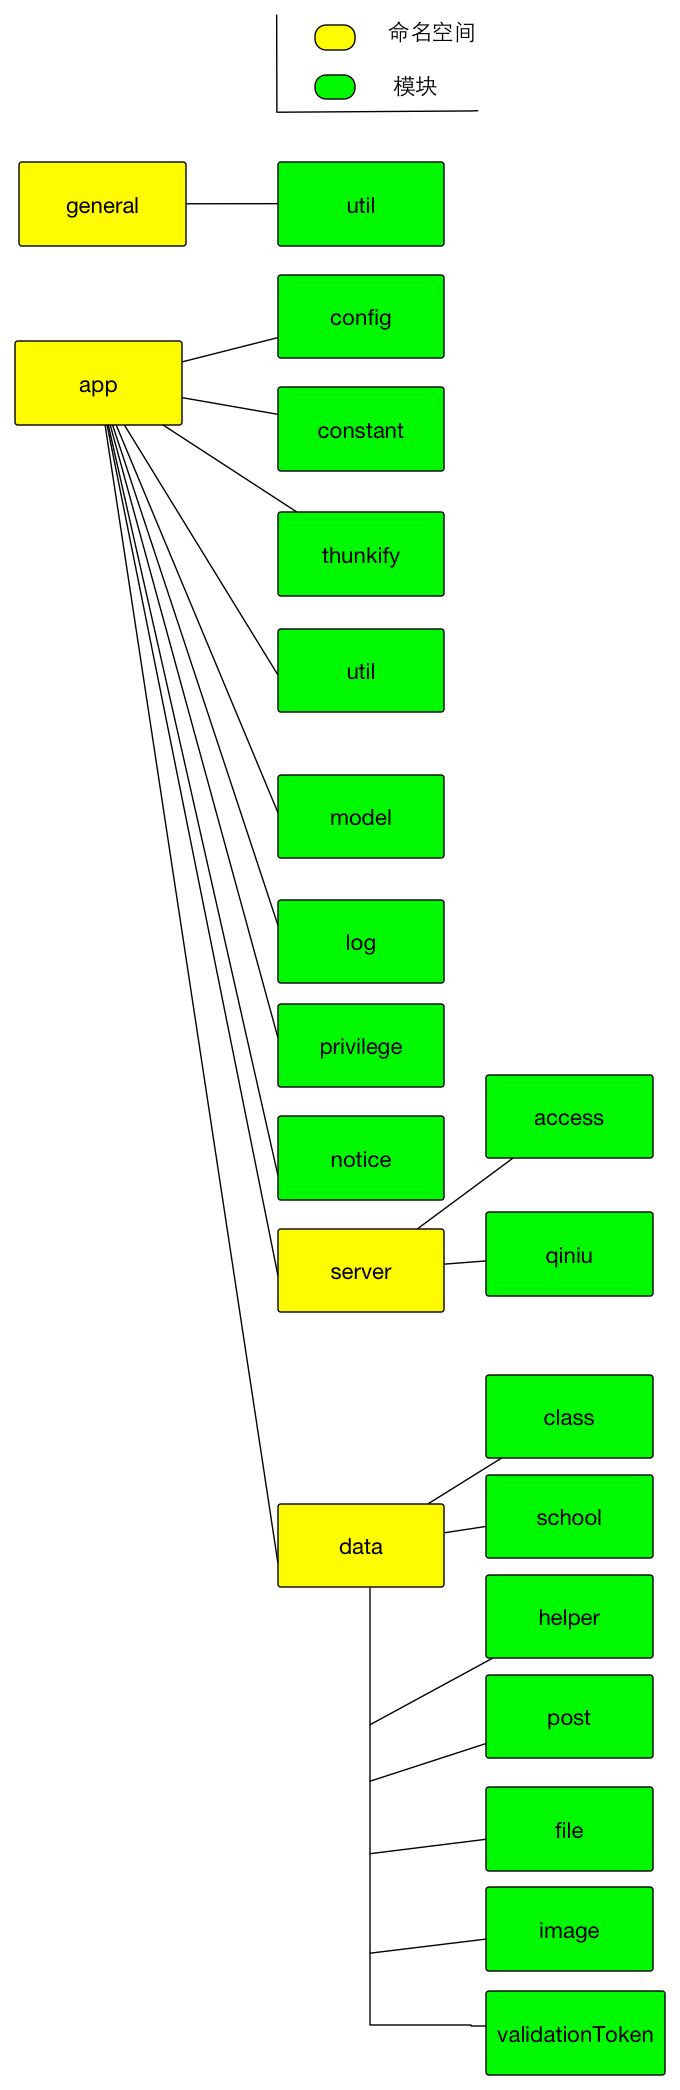
\includegraphics[width=0.35\textwidth]{modules_tree.jpg}
	\figcaption{Node 模块关系}
	\label{fig: modules}
\end{figure}

\newpage
\subsection{系统每个模块作用}

\begin{description}
	\item[general.util] 放一些任何地方都可能被重用到,且与该应用关系不大的代码
	\item[app.config]  配置信息
	\item[app.constant] 使用的一些常量
	\item[app.model] 数据库定义
	\item[app.thunkify]   数据库的一个浅层包装, 对数据库部分操作提供promise形式的接口

	\item[app.util] 一些很多地方都可能被重用到,但与该应用场景耦合度较高的代码
	
	\item[app.log] 日志系统
	
	\item[app.notice] 发短信,邮件,手机端Push Notification通知系统
	
	\item[app.privilege] 系统对于权限相关的操作
	
	\item[app.server.access] 系统服务器的验证(登陆,注册)系统
	
	\item[app.server.qiniu] 系统使用的七牛云服务操作
	
	\item[app.data.class] 对于数据库中班级的抽象层
	
	\item[app.data.school] 对于数据库中学校的抽象层
	
	\item[app.data.helper] 对于数据库中帮手的抽象层
	
	\item[app.data.file] 对于数据库中文件的抽象层
	
	\item[app.data.image] 对于数据库中相册的抽象层
	
	\item[app.data.validationToken] 对于数据库中验证的抽象层
	
	
\end{description}



\subsection{系统模块设计要点}


\begin{enumerate}
	\item 要保证这些modules直接高内聚, 低耦合,直接互相依赖度低, 都可以被当做独立的工具使用
	\item 使用 Github organization, 每个modules都对应organization中的一个 repository. 
	\item 将每个repository都发布为私有的 NPM 模块, 这样可以在任何地方使用 npm install 来进行模块的安装, 使得该应用的每个部分都成为独立的工具
	
	\item 最上层的程序应当很短,只是调用相应模块, 创建服务器并将模块注入其中, 之后服务器开始运行
	
\end{enumerate}












